\section{\uppercase{Method}}
\label{sec:method}
\subsection{A Shared Artifact Contract}
A public profile specifies the model, observable representation, numerical rules, coder and budget. The sender seals canonical source bytes once and encodes the packet into carrier $y$. The receiver obtains only saved $y$, the profile, shared context and encryption key. Source bytes/digests, sender identifiers, ranks, packets and latent codes are excluded. Figure~\ref{fig:examples} shows both directions using the first manifest-ordered fixed-rank example in each direction. Panel A carries canonical image pixels through saved text. Panel B carries literal text through a saved PNG.\aifootnote

\begin{figure*}[t]
\centering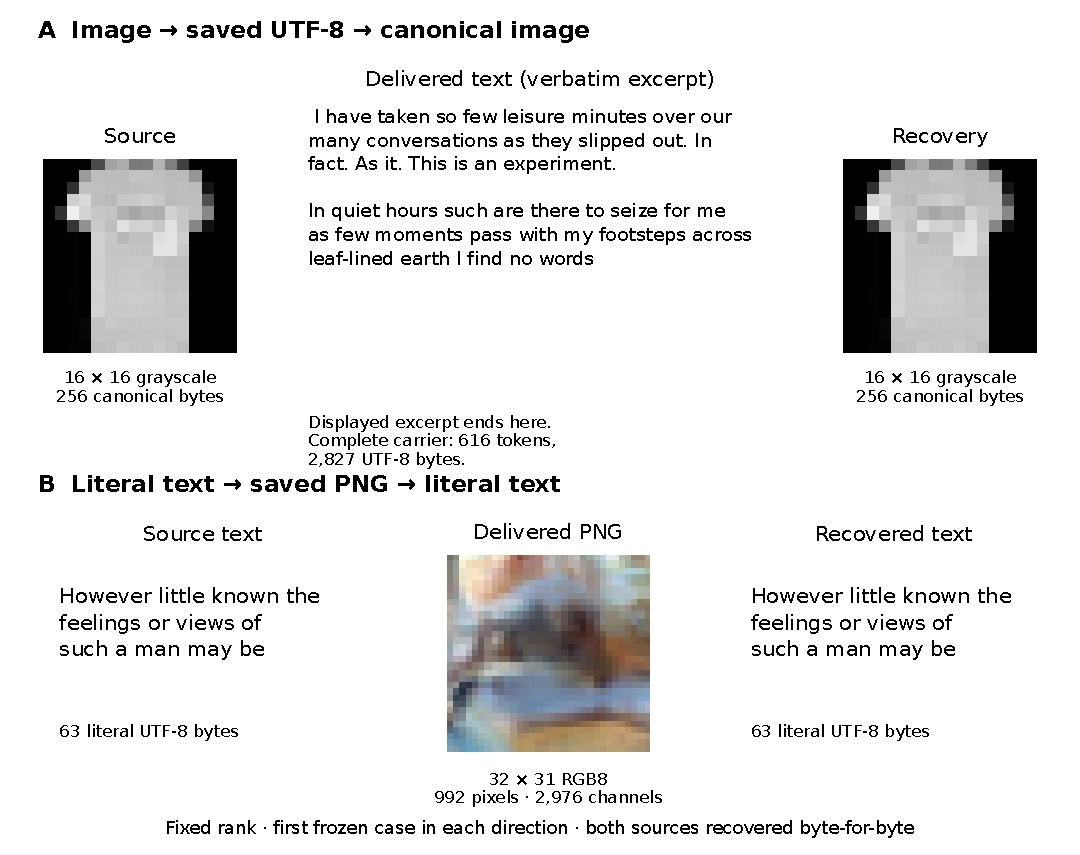
\includegraphics[width=\textwidth]{figures/figure1_transport_submission.pdf}
\caption{Actual artifacts selected by the first fixed-rank case in each direction. A transports a canonical $16\times16$ grayscale array through the displayed verbatim excerpt of a 616-token, 2,827-byte UTF-8 carrier. Recovery restores all 256 canonical pixels, not an arbitrary image file. B shows the complete 63-byte source/recovered messages and actual $32\times31$ RGB PNG. Pixels use nearest-neighbor display. Each fresh receiver uses its saved carrier, model/profile, shared context and key. The PNG conditioning row is withheld from the carrier and prepended internally. Authentication and separate source-byte equality both pass.}
\label{fig:examples}
\end{figure*}

Images are canonical $16\times16$ grayscale arrays of unsigned eight-bit pixels, 256 bytes in row-major order. Exact recovery restores this preprocessed array, not the larger original image or its container. Text is 32--128 literal UTF-8 bytes without normalization, added newlines or replacement decoding.

The plaintext header contains version (one byte, 1), kind (one byte, 1 for text or 2 for grayscale), source length (two bytes), width (two bytes) and height (two bytes). Multibyte integers are unsigned big-endian. A 256-byte slot follows, with source bytes first and zero padding. Text dimensions are zero. Image dimensions are $16\times16$. No MIME field or payload sidecar is added.

AES-256-GCM \cite{gcm} authenticates and encrypts the entire header and slot using a fresh random key and a unique random 12-byte nonce. The associated data are the exact ASCII bytes \texttt{ImageCalgacus/packet/v1}, with no newline. The carried packet is
\begin{equation}
\begin{aligned}
P&=\text{nonce}\,\|\,\text{ciphertext}\,\|\,\text{tag},\\
|P|&=12+264+16=292\ \text{bytes}.
\end{aligned}
\label{eq:packet}
\end{equation}
The known 2,336-bit target avoids circular framing around an encrypted length. After authentication the parser validates type, length, dimensions, UTF-8 and all padding bytes, returning no plaintext on failure. The evaluator checks equality separately. Authenticated encryption protects content under its usual assumptions, not the channel's existence.

One immutable packet is shared across the paired methods in a payload/context group. Reusing that ciphertext is not a new encryption under a reused nonce. Keys and nonces come from operating-system randomness, independently of sampling seeds. Continuation retains the sealed packet without supplying it to receivers.

\subsection{Observable Conditional Distributions}
At position $t$, the backend supplies eligible symbols $E_t$, normalized probabilities $q_t(v)$ and a deterministic rank order. Conditioning includes the shared context and all preceding observed symbols, including skips and completion. Text ranks use descending logits, with ascending token identifier breaking exact ties. Image ranks use descending log probability, then ascending channel value. Probability bookkeeping uses float64, stable normalization and ascending-identifier summation. NaN, positive infinity, empty support and invalid normalization are explicit failures. Numerical zero mass is excluded and the remaining distribution renormalized, without an added probability floor. Ordinary sampling is temperature-one inverse-CDF sampling in identifier order, with no nucleus truncation.

For text, the model is Llama 3 8B Instruct \cite{llama3}, not an image model. Let $T$ tokenize bytes without BOS insertion or special-token interpretation, and let $D$ return exact bytes without cleanup. Given carrier prefix $s$, each candidate $v$ must satisfy
\begin{equation}
T\bigl(D(s\mathbin{\|}[v])\bigr)=s\mathbin{\|}[v].
\label{eq:consistent}
\end{equation}
The pool contains the top 256 model tokens \emph{before} filtering. Special or control tokens, empty renderings and invalid UTF-8 are excluded. Equation~\ref{eq:consistent} is checked on the complete carrier prefix, not a prompt/carrier concatenation. The model sees one BOS followed by separately tokenized prompt bytes and carrier identifiers, without a chat template. The receiver tokenizes the delivered file separately, checks exact byte round-trip equality, and replays the same prefix tests. Payload positions, gate skips, arithmetic steps and the 32-token ordinary tail all obey this rule.

For PNG carriers, PixelCNN++ \cite{pixelcnn} models a native $32\times32$ RGB canvas. A shared $1\times32$ RGB row occupies the first row. Only the remaining 31 rows are delivered, giving 992 pixels or 2,976 channel values. Each channel value in $\{0,\ldots,255\}$ is observable. Generation and replay use raster order, with R then G then B within each pixel. The receiver reads an eight-bit RGB PNG without palette conversion, alpha compositing or color transformations and prepends the shared row internally.

The network predicts ten mixture weights, channel means, log scales and RGB dependency coefficients per pixel, not 256 independent categorical logits. Let $f_{k,C}$ denote a discretized logistic component mass for channel $C$. For normalized intensity $z(v)=2v/255-1$, component probabilities are logistic CDF differences over half-bin width $1/255$, with infinite tails at 0 and 255. Log scales are lower bounded by $-7$ and dependency coefficients use $\tanh$. We evaluate the discrete masses in float64 rather than using the upstream continuous sampler or its small-density fallback.

Channels require mixture posteriors, not independent marginals. After red, weights satisfy $w_k^R\propto w_k f_{k,R}(r)$. Green uses normalized $w^R$ and mean shift $a_{RG}z(r)$. After green, $w_k^{RG}\propto w_k^R f_{k,G}(g\mid r)$. Blue uses normalized $w^{RG}$ with mean shift $a_{RB}z(r)+a_{GB}z(g)$. One network forward per visible pixel supplies all parameters, reused within that pixel. Causal checks establish that unobserved pixels do not alter them.

\subsection{Three Packet Coders}
\label{sec:coders}
\paragraph{Fixed rank.}
Each packet byte yields its high nibble and then low nibble. A nibble $d\in\{0,\ldots,15\}$ selects eligible rank $d+1$. Exactly $292\times2=584$ positions carry the packet. The receiver inverts observed ranks into bytes and stops by this fixed count. Fewer than 16 eligible symbols while the packet is pending causes a support failure, not a smaller alphabet.

\paragraph{Entropy-gated rank.}
The same four-bit operation is applied only if
\begin{equation}
H(q_t)=-\sum_{v\in E_t}q_t(v)\log_2q_t(v)>\tau.
\end{equation}
Otherwise the sender samples ordinarily and consumes no packet bits. The receiver recomputes the strict comparison from the observed prefix, so no gate trace is transmitted. Separate thresholds were calibrated from ordinary development traces and frozen at $0.5983972524635524$ bits for text and $3.2159513527579326$ bits for channels. They were not adjusted after failures.

\paragraph{Arithmetic A1.}
We independently implement a finite-precision arithmetic comparator following Neural Linguistic Steganography \cite{ziegler}. A1 identifies our framing adaptation, not a new security construction. It starts with the half-open interval $[0,2^{32})$. At width $R$, retain symbols with $q_t(v)\geq1/R$ and at least the top $\min(2,|E_t|,R)$ symbols. Renormalize retained probabilities, round bin widths to nearest integer with ties to even, truncate before the first cumulative overflow, and assign residual width to the first symbol. Remove zero-width bins. Positive widths must sum to $R$.

The next 32 source bits, zero-extended only beyond the packet, select the interval bin. Sender and receiver emit the common leading bits of its lower bound and upper bound minus one, then shift the interval accordingly. A zero-bit step updates the interval and consumes carrier capacity. Packet completion occurs at the first common-prefix emission reaching 2,336 bits. At most 31 emitted suffix bits are checked to be zero and discarded. There is no end token, final-artifact endpoint dump or implicit flush during ordinary completion. The receiver needs no sender offset to determine progress.

This framing differs from the reference's final-token endpoint handling. A1 can stagnate when a narrow interval straddles a leading-bit boundary and quantization retains one bin, leaving that interval unchanged. Its precision and stopping rules remain fixed. Capacity exhaustion is an outcome, but desynchronization is an implementation defect. An incomplete packet prefix is not authenticated delivery.

\subsection{Stopping, Completion and Conditional Inversion}
All text carriers have a 2,048-token cap. After packet completion the sender must add exactly 32 ordinary tokens within that cap. A packet completing too late for the tail is packet-complete but carrier-incomplete. An unfinished packet is not truncated early to reserve a tail. PNG generation always completes all 2,976 channels after the packet stop, including any remainder of a partially used RGB pixel. No packet is stored in PNG metadata or appended bytes.

Inversion follows inductively when both endpoints reconstruct the same distribution and coder transition from each observed prefix. Equation~\ref{eq:consistent} supplies the text invariant, and lossless pixel equality supplies the PNG invariant. The fixed packet size supplies framing. Sufficient support and finite termination remain necessary conditions.

Senders exit before fresh receivers start. Their input directories contain only carrier, profile, context and key, with model assets separately available. Evaluation follows receiver exit. Reports distinguish packet and carrier completion, receiver recovery, authentication, carrier conformance and source equality.
